\section{Animation}


\subsection{Sprites}

De animatie van de kat wordt bekomen door het snel achter elkaar tekenen van delen van een sprite sheet. Deze sheet bevat in dit geval 8 frames, zie figuur \ref{fig:cat}. De breedte van de sheet zal door het aantal frames worden gedeeld om zo met een "draw" methode elke deel appart en achter elkaar te displayen. Op deze manier creërt men de illusie van beweging op een zeer simpele manier. In dit geval loopt de kat naar rechts maar met een spiegel methode kan de andere richting bekomen worden.

\begin{figure}[h]
\centering
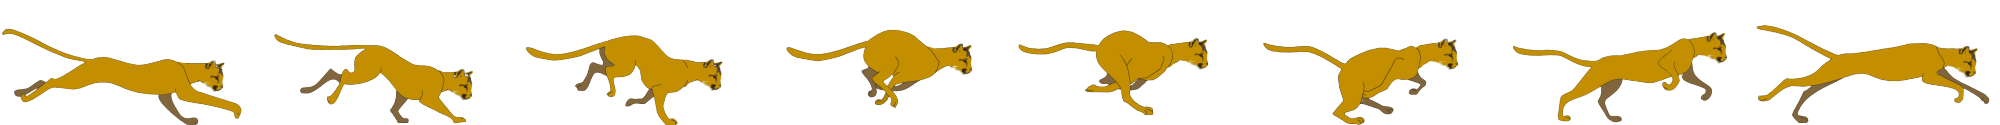
\includegraphics[scale=0.3]{img/cat2.png}
\caption{Kat sprite sheet \cite{catsprite}}
\label{fig:cat}
\end{figure}




\subsection{Delaunay}

Voor de animatie wordt gebruik gemaakt van de reeds geschreven delaunay triangulatie. Deze zal het pad vormen waarover de kat zal lopen. Wanneer de kat zich dicht genoeg bij het endPoint bevindt zal deze de firstPoint worden en zullen de buren ervan opgevraagd worden. Er zal willeukeurig een punt worden gekozen als nieuw endPoint. Dit punt kan niet het firstPoint van de vorige beweging zijn. Dit wil zeggen dat de animatie nooit terug op zijn stappen komt. Enkel als de triangulatie een rechte lijn vormt zal de sprite op en neer lopen. 

